\pagestyle{empty}%	清空页面风格

\begin{tikzpicture}[remember picture, overlay]
    \node[anchor=center] (title) at ([yshift=20em] current page.center){\fontsize{32}{32}\textsf{AJ-Note1}};
    \node[anchor=center] (author) at ([yshift=-2em] title.south){\fontsize{14}{14}\textsf{Written by An}};
    \node[anchor=center] (date) at ([yshift=-2em] author.south) {\fontsize{14}{14}\textsf{Compile date: \today}};
\end{tikzpicture}


\clearpage % Inner page
\vspace*{5em}

\begin{center}
    Repository address: \url{https://github.com/PupilEarthquake/Aj_Note1} \\
    Home page: \url{https://www.xiaorp.xyz/} \\
\end{center}

\vfill

\begin{tabular*}{\textwidth}{ccc}
    
\includegraphics{config/ccby.png}
    & \begin{minipage}[b]{0.6\textwidth}
        \small This work is licensed under Creative Commons Attribution 4.0 International license. Access \url{http://creativecommons.org/licenses/by/4.0/} view the license agreement.
    \end{minipage}
\end{tabular*}
\cleardoublepage


% 废话页
\vspace*{10em}
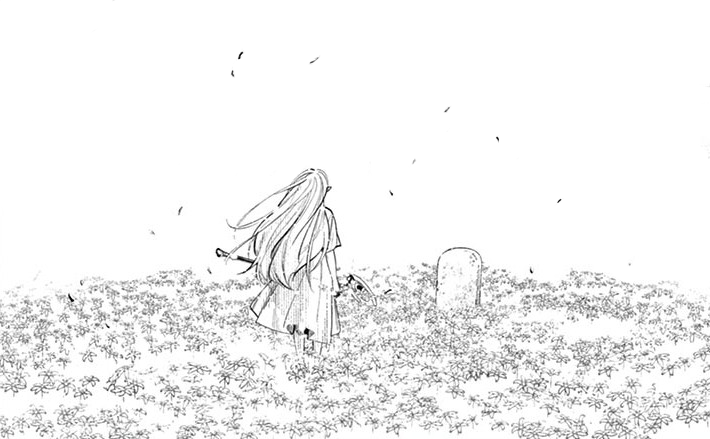
\includegraphics[width=\textwidth]{config/frieren.png}
\begin{center}
    \textit{The era of humanity has arrived.}
\end{center}

% 目录
\cleardoublepage

\pagestyle{fancy}		% 复原页面风格为 fancy
\pagenumbering{roman}	% 页码复原为小写罗马字母

\setcounter{page}{1}
\thispagestyle{empty}
\addtocontents{toc}{\protect\thispagestyle{empty}}

\tableofcontents